\documentclass[a4paper,11pt]{article}
\newcommand\tab[1][0.6cm]{\hspace*{#1}}
\usepackage{mlsubmit}

\begin{document}

\initmlsubmision{1}                              					% assignment number
								{Raktim Mitra}      						           		% your name
								{150562}																		% your roll number

\begin{mlsolution}
\subsection*{Solution for $d_U$:}
	Let, $\mathbf{z_1}=(x_1,y_1)$ and $\mathbf{z_2}=(x_2,y_2)$ then $d_U(\mathbf{z_1,z_2}) = \langle(z_1 - z_2),U(z_1,z_2) \rangle$. Upon calculating the inner produc we get:
	
	$d_U(\mathbf{z_1,z_2}) = 3(x_1 - x_2)^2 + (y_1 - y_2)^2$
	
	The decision boundary is the locus of points $\mathbf{z}$ with equal distance from both $\mathbf{z_1}$ and $\mathbf{z_2}$. i.e.
	
\tab $3(x_1 - x)^2 + (y_1 - y)^2 = 3(x_2 - x)^2 + (y_2 - y)^2$

Putting $\mathbf{z_1} = (1,0)$ and $\mathbf{z_2} = (0,1)$ :

\tab $3(x-1)^2 + y^2 = 3x^2 + (y-1)^2$

$\implies -6x - 1 = -2y + 1$

$\implies 2y = 6x - 2$

$\implies y = 3x - 1$ [Answer]


\begin{figure}[th]%
\centering

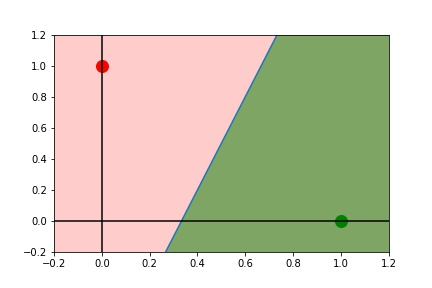
\includegraphics[width=0.5\columnwidth]{q1/d1.jpg}%
\hfill
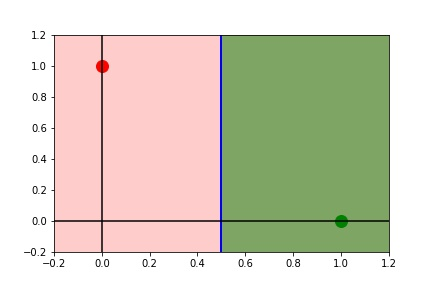
\includegraphics[width=0.5\columnwidth]{q1/d2.jpg}%
\caption{Learning with Prototypes: The figure on the left shows the decision boundary with $d_U$ distance metric. The decision boundary is $y= 3x-1$. The figure on the right shows the decision boundary with $d_V$ distance metric. The decision boundary is $x = 0.5$. }
\label{fig:proto}%
\end{figure}
\subsection*{Solution for $d_V$:}
	Let, $\mathbf{z_1}=(x_1,y_1)$ and $\mathbf{z_2}=(x_2,y_2)$ then $d_V(\mathbf{z_1,z_2}) = \langle(z_1 - z_2),V(z_1,z_2) \rangle$. Upon calculating the inner product we get:
	
	$d_V(\mathbf{z_1,z_2}) = (x_1 - x_2)^2 $ (Only depends on x !)
	
	The decision boundary is the locus of points $\mathbf{z}$ with equal distance from both $\mathbf{z_1}$ and $\mathbf{z_2}$. i.e.
	
\tab $(x_1 - x)^2  = (x_2 - x)^2$

Putting $\mathbf{z_1} = (1,0)$ and $\mathbf{z_2} = (0,1)$ :

\tab $3(x-1)^2  = 3x^2 $

$\implies 2x = 1$

$\implies x = \frac{1}{2}$ [Answer]


\end{mlsolution}

\begin{mlsolution}

We can incorporate the constraint into the prior distribution by setting prior probaility to 0 if $\norm{\vw} > r$ . We also want \textbf{log(P(w))} to vanish since  we want a MAP estimate that matches the given estimation function which resembles only an MLE, i.e. a MAP with constant prior. so for  $\norm{\vw} \leq r$ we set the prior to be uniform distribution. The value of this constant in the probability density function is $\frac{1}{\rho}$ where $\rho$ is the volume of hipersphere of radius r. This preserves the total probability to 1. Therefore:

\begin{center}
$\textbf{PDF P(w)} = \frac{1}{\rho}$ $if \norm{\vw} \leq r$, 0 otherwise
\end{center}

The likelihood $\mathbf{P(}y^i$ $|$ $\mathbf{w,X_i)}$ remains same as we use for the unconstrained version.
\begin{center}
\textbf{PDF} $\mathbf{P(}y^i$ $|$ $\mathbf{w,X_i)}$ $= \frac{1}{\sqrt{2\pi}\sigma}e^{-\frac{(y^i - \langle\mathbf{w,X^i\rangle})^2}{2\sigma^2}}$\\[1 em]

and $\mathbf{P( y}$ $|$ $\mathbf{w,X)} = \prod_{i=1}^{n} \mathbf{P( y^i}$ $|$ $\mathbf{w,X^i)}$ \\[1 em]
\end{center}

This works because when  $\norm{\vw} \leq r$ the MAP estimation reduces to 
\begin{center}
$\arg\min_{\mathbf{w}} \sum_{i=1}^n(y^i - \ip{\vw}{\vx^i})^2$
\end{center}

Otherwise the cost function shoots up as $-log(\mathbf{P(w)}) = - log(0)$ goes to infinity.

There for the MAP estimation becomes
\begin{center}
$\arg\min_{\mathbf{w}} \sum_{i=1}^n(y^i - \ip{\vw}{\vx^i})^2$ where $\norm{\vw} \leq r$\\[1em]

-----
\end{center}
%
%%\begin{figure}[th]%
%\centering
%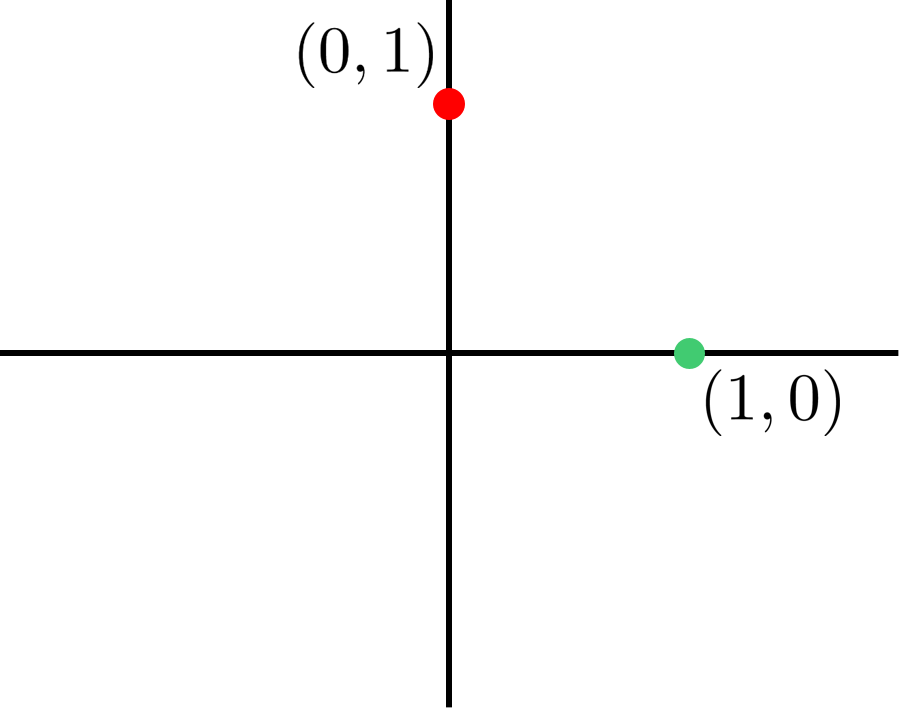
\includegraphics[width=0.5\columnwidth]{proto_blank.png}%
%\hfill
%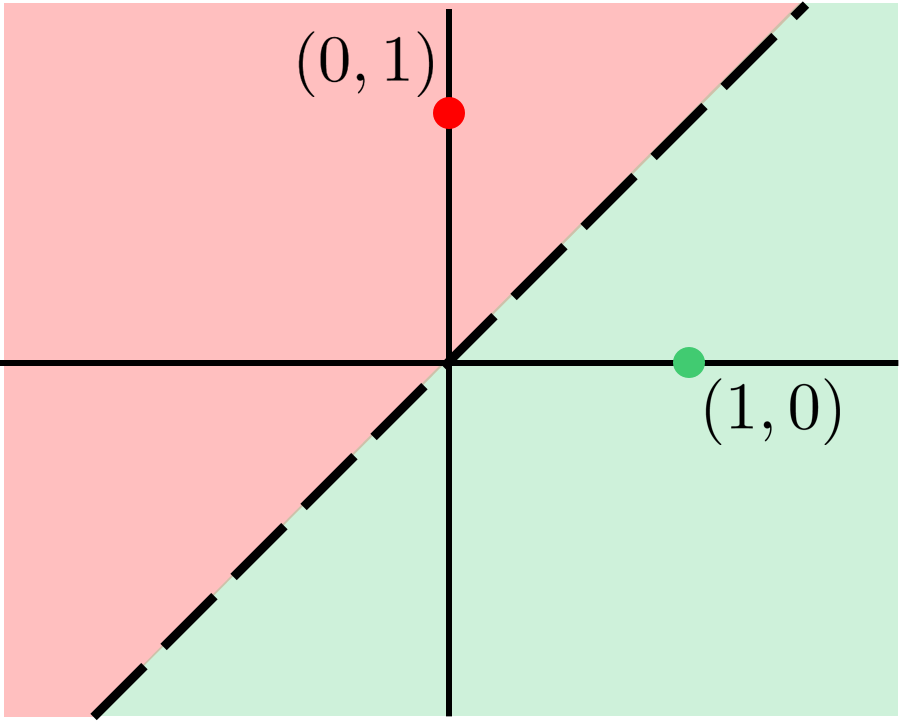
\includegraphics[width=0.5\columnwidth]{proto_euclid_sample.png}%
%\caption{Learning with Prototypes: the figure on the left shows the two prototypes. The figure on the right shows what the decision boundary if the distance measure used is $d(\vz^1,\vz^2) = \norm{\vz^1-\vz^2}_2$, for any two points $\vz^1,\vz^2 \in \bR^2$. The decision boundary in this case is the line $y = x$.}%
%\label{fig:proto}%
%\end{figure}

\end{mlsolution}

\begin{mlsolution}
Likelihood distribution:
\begin{center}
$\mathbf{P( y^i}$ $|$ $\mathbf{w,X^i)} = \frac{1}{\sqrt{2\pi}\rho}e^{-\frac{(y^i - \langle\mathbf{w,X^i\rangle})^2}{2\rho^2}}$\\[1em]

and $\mathbf{P( y}$ $|$ $\mathbf{w,X)} = \prod_{i=1}^{n} \mathbf{P( y^i}$ $|$ $\mathbf{w,X^i)}$ \\[1 em]

\end{center}

Prior Distribution:
\begin{center}
$\textbf{P(w)} = \prod_{i=1}^{d} \mathbf{P(w_i)}$ \\[1 em]

where, $\mathbf{P(w_i)} =  \frac{1}{\sqrt{2\pi}\sigma_i}e^{-\frac{ \mathbf{{w_i}^2}}{2{\sigma_i}^2}}$ 
\end{center}

Explanation:
\begin{center}
$-log(\mathbf{P( y}$ $|$ $\mathbf{w,X)}) = \sum_{i = 1}^{n} -log(\mathbf{P(y^i}$ $|$ $\mathbf{w,X^i)})$ \\[1em]
$= \sum_{i = 1}^{n} \frac{(y^i - \langle\mathbf{w,X^i\rangle})^2}{2\rho^2}$ (ignoring log of constants)\\[2em]


$-log(\mathbf{P(w)}) = \sum_{i = 1}^{d} -log(\mathbf{P(w_i)})$ \\[1em]
$= \sum_{i = 1}^{d} \frac{\mathbf{w_i}^2}{2{\sigma_i}^2}$ (ignoring log of constants)
\end{center}

So, multiplying both with $2\rho^2$ MAP estimation becomes:
\begin{center}
$\arg\min_{\mathbf{w}} \sum_{i=1}^n(y^i - \ip{\vw}{\vx^i})^2 + \sum_{i = 1}^{d} \frac{\mathbf{\rho}^2}{{\sigma_i}^2}\mathbf{{w_i}^2}$ 
\end{center}

Putting $\frac{\mathbf{\rho}^2}{{\sigma_i}^2} = \alpha_i$ we get the required form of the optimisation problem :
\begin{center}
	$\arg\min_{\mathbf{w}} \sum_{i=1}^n(y^i - \ip{\vw}{\vx^i})^2 + \sum_{i = 1}^{d} \alpha_i\mathbf{{w_i}^2}$
\end{center} 
let, $\textbf{A}$ be a $d$ x $d$ diagonal matrix where diagonal entries are $\alpha_i's$ and $\mathbf{w}$ is $d$ x $1$ then $\sum_{i = 1}^{d} \alpha_i\mathbf{{w_i}^2}$ can be written as $\mathbf{w^TAw}$. \textbf{X} is $n$ x $d$, i.e. each row is a training example, then $\sum_{i=1}^n(y^i - \ip{\vw}{\vx^i})^2$ can be written as $\langle{\mathbf{y-Xw},\mathbf{y-Xw}}\rangle$ which is $\mathbf{(y-Xw)^T(y-Xw)}$.
Therefore the optimisation function becomes:
\begin{center}
$\mathbf{y^Ty + w^tX^TXw - w^TX^Ty - y^TXw + w^TAw}$ \\ = $\mathbf{y^Ty + w^tX^TXw - 2w^TX^Ty + w^TAw}$ (since $w^TX^Ty = y^TXw = \langle\mathbf{Xw},\mathbf{y}\rangle$)
\end{center}
to find minimum set, derivative w.r.t \textbf{w} to 0: 
\begin{center}
	$\mathbf{0 + 2X^TXw - 2X^Ty + 2Aw} = 0$\\
	$\implies \mathbf{(X^TX + A)w = X^Ty}$\\
	$\implies \mathbf{\widehat{w} = {(X^TX + A)}^{-1}X^Ty}$ [Answer]
\end{center}
\end{mlsolution}

\begin{mlsolution}
\begin{align*}
\bc{\widehat\vW, \{\hat\xi_i\}} = \underset{\vW,\bc{\xi_i}}{\arg\min}&\ \sum_{k=1}^K\norm{\vw^k}_2^2 + \sum_{i=1}^n\xi_i\\ 
\text{s.t.} &\ \ip{\vw^{y^i}}{\vx^i} \geq \ip{\vw^k}{\vx^i} + 1 - \xi_i, \forall i, \forall k \neq y^i\qquad\qquad{(P1)}\\
&\ \xi_i \geq 0, \text{ for all } i
\end{align*}
Looking at the constraints, we get $\xi_i \geq max(0,\ip{\vw^k}{\vx^i} - \ip{\vw^{y^i}}{\vx^i} + 1) \text{ for all i and }\text{for all k} \neq y^i$ . Which is equevalent to $\xi_i \geq max(0,1 + \max_{k \neq y}\veta^i_k - \veta^i_y) \text{ for all i. In notations given in problem}$ 
i.e. $\xi_i \geq [1 + \max_{k \neq y}\veta^i_k - \veta^i_y]_+ \text{ for all i.} $ \\[0.5 em]
\underline{\textbf{Proof of equevalence :}}\\[0.1em]

\textbf{P2 $\implies$ P1:}

\tab Let, $\mathbf{\widehat{W}}$ is a soution of \textbf{P2}. $\hat\xi_i = [1 + \max_{k \neq y}\hat\veta^i_k - \hat\veta^i_y]_+ \text{ for all i}$,where $\hat\veta^i = \ip{\widehat{\vW}}{\vx^i}$  gives optimal solution of \textbf{P1},because once \textbf{P1} reaches $\widehat{\vW}$, there is no way $\xi_is$ can be reduced from $\hat\xi_is$. Therefore, there exists $\{\hat\xi_i\}$ such that $\widehat{\textbf{W}}$,$\{\hat\xi_i\}$ is a solution of \textbf{P1}.\\[0.1em]

\textbf{P1 $\implies$ P2:}

	\tab Let,  $\widehat{\textbf{W}}$,$\{\hat\xi_i\}$ be an optimal solution of \textbf{P1}. That means,  $\xi_i \geq max(0,\ip{\vw^k}{\vx^i} - \ip{\vw^{y^i}}{\vx^i} + 1) \text{ for all i and }\text{for all k}$, which is equevalent to  $\hat\xi_i \geq [1 + \max_{k \neq y}\hat\veta^i_k - \hat\veta^i_y]_+ \text{ for all i}$. 
	
	\tab Claim: $\hat\xi_i = [1 + \max_{k \neq y}\hat\veta^i_k - \hat\veta^i_y]_+ \text{ for all i}$. 
	
	\tab Proof: Otherwise $\hat\xi_i > [1 + \max_{k \neq y}\hat\veta^i_k - \hat\veta^i_y]_+ \text{ for all i}$. But in that case we can choose a smaller $\xi_i$ which will minimise the objective function further while abiding by the connstraints. This contradicts the fact that $\widehat{\textbf{W}}$,$\{\hat\xi_i\}$ is optimum.
	
	\tab Therefore, by replacing $\xi_is$ with $[1 + \max_{k \neq y}\veta^i_k - \veta^i_y]_+ \text{ for all i}$ i.e. $\ell_\text{cs}(y^i,\veta^i)$, we get that \textbf{P1} is  restructured to \textbf{P2} while $\widehat{\textbf{W}}$ remains optimal. 
	
	\tab This proves $\widehat{\vW}$ is an optimal solution of Problem \textbf{P2}.
	
	Hence, P1 and P2 are equevalent optimisation problems. [Proved]
	
\end{mlsolution}
\begin{mlsolution}

To prove that $\textbf{g}$ is a subdifferential of f at \textbf{w}, we show that for every $\textbf{z} \in \mathbb{R}^d$:
	$$ f(\textbf{z}) \geq f(\textbf{w}) + \langle\textbf{g}, \textbf{z} - \textbf{w}\rangle$$\\
We can write $\vg$ as $\textbf{g} = \sum\limits_{i \in S} -y^i\textbf{X}^i$ where $S$ is the set of $i's$ such that $y^i\langle\textbf{w}, \textbf{X}\rangle < 1$\\
	\begin{center}		
		$\textbf{w}^T\textbf{g} = \sum\limits_{i \in S} -\textbf{w}^T y^i\textbf{X}^i$\\
		%\intertext{Since we are working on real numbers in LHS, $\textbf{w}^T\textbf{g} = \textbf{g}^T\textbf{w}$}
		$\implies \textbf{g}^T\textbf{w} = \sum\limits_{i \in S} -y^i\textbf{w}^T\textbf{X}^i$ (since $\mathbf{w^Tg = g^Tw = \langle w,g\rangle}$)\\
		$\implies f(\textbf{w}) + \langle\textbf{g}, \textbf{z} - \textbf{w}\rangle = f(\textbf{w}) + \textbf{g}^T\textbf{z} - \textbf{g}^T\textbf{w}$\\
				$= \sum\limits_{i \in S}^{n}[1 - y^i \langle\textbf{w}, \textbf{X}^i\rangle] + \sum\limits_{i \in S} -y^i\textbf{z}^T\textbf{X}^i + \sum\limits_{i \in S} y^i\textbf{w}^T\textbf{X}^i$\\
				$= \sum\limits_{i \in S} 1 - y^i \langle \textbf{z}, \textbf{X}^i\rangle$
	\end{center}
To complete the proof we need to consider two cases:
	\begin{enumerate}
	
		\item $y^i \langle \textbf{z},\textbf{X}^i\rangle < 1$ Then the term's contribution in RHS is greater than 0. By definition,it is a part of f(z).
		\item $y^i \langle \textbf{z},\textbf{X}^i\rangle \geq 1$ Then contribution is negative. This term reduces the RHS sum only.Hence does not contribute to f(z).
	\end{enumerate}
	$\therefore$ f(z) is sum of all positive quantities in RHS of the expression and some other positive terms. Hence:
	\begin{center}
				$$ f(\textbf{z}) \geq \sum\limits_{i \in S} 1 - y^i \langle \textbf{z}, \textbf{X}^i\rangle$$
			$$\implies f(\textbf{z}) \geq f(\textbf{w}) + \langle\textbf{g}, \textbf{z} - \textbf{w}\rangle$$ [Proved]
	\end{center}
\end{mlsolution}
\begin{mlsolution}
\subsection*{Part 1:}
Test Error for 5 different k values:\\
\tab k = 1 \tab \tab 24.075\%\\
\tab k = 2 \tab \tab 21.44\%\\
\tab k = 3 \tab \tab 19.19\%\\
\tab k = 5 \tab \tab 17.71\%\\
\tab k = 10\tab \tab 16.795\%\\

\begin{figure}[th]
\centering
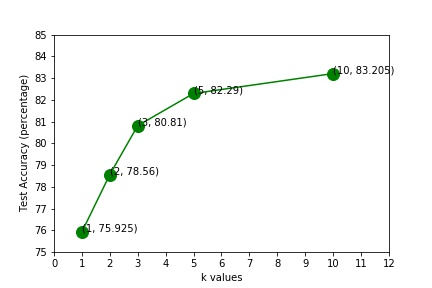
\includegraphics[width=\columnwidth]{q6_1.jpg}
\caption{Plot showing test accuracy for k values \{1,2,3,5,10\}}
\label{fig:proto}
\end{figure}
\textbf{Observation:}
 As expected, number of neighbour points considered increases as we go from 1 to 10. The decision for each point takes into account more number of points, leading to minimising chanes of error.

\subsection*{Part 2:}
  I devided the train data in 8:2 ratio(train and validation) and calculated the accuracy for k = 10 to 100 with steps of 5. I found high values around 15,20. Then I reran the validation with k = 15 to 24 and found highest value at 21.

Therefore tuned value of k is 21.

\subsection*{Part 3:}
Learned suitable metric with lmnn, used 6000 data points and 3000 iterations. Although it did not converge but as the plot shows the objective was changing very slowly after around 1000 iterations. Therefore we can say the learned metric is good enough.
\begin{figure}[th]
\centering
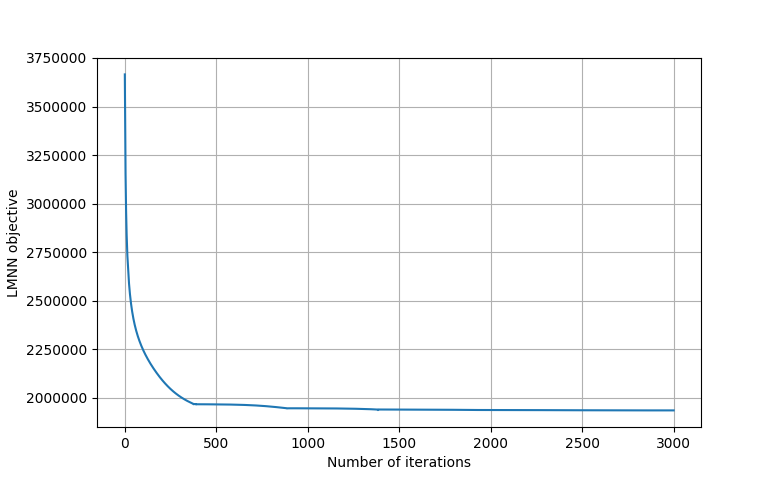
\includegraphics[width=\columnwidth]{Figure_1.png}
\caption{Plot showing lmnn objective w.r.t. number of iterations for k = 21}
\label{fig:proto}
\end{figure}

Using the learnt Metric and K = 21 the test accuracy is \textbf{83.975\%}

\end{mlsolution}	
\end{document}
